\chapter{Design}
\label{Design}

    \section{System Architecture}
    \label{des:system_arch}
    With the requirements complete, the next step was to create an architectural diagram of the system that outlined the different components, functions and how they would connect with one another. Designing the architecture went through an iterative process of adding more detail and components until a detailed enough design was built. The initial system architecture can be seen in Figure \ref{fig:architecture_orginal} and consisted of a linear path in which articles were found, processed and put into the database. Then the resulting sentences from these articles were processed. There also existed a stock prediction component to make the future price predictions.
    
    \begin{figure}[!h]
        \centering
        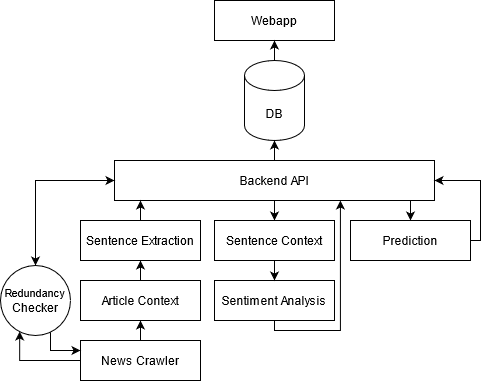
\includegraphics[width=0.7\textwidth]{images/upload/Architecture_origonal.png}
        \caption{Original Architecture}
        \label{fig:architecture_orginal}
    \end{figure}
    
    As work on the project continued it became clear that improvements could be made to original design, shown in Figure \ref{fig:architecture_orginal}. The components were too tightly coupled to one another, since each depended on one another to manage the flow of data and communication. Additionally, since all components attempted to access the database simultaneously it could potentially cause strain on the backend API and database. To remedy these concerns the system architecture was revised to better tackle these issues. 
    
    \begin{figure}[!h]
        \centering
        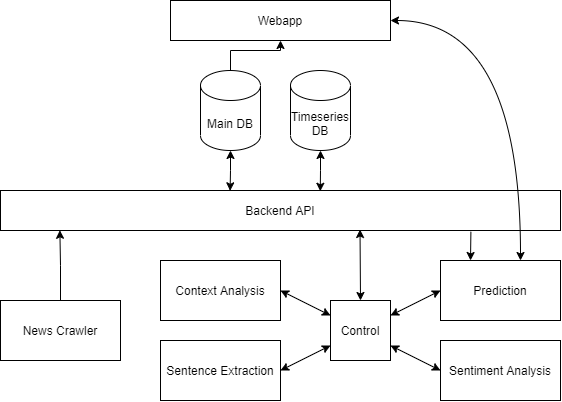
\includegraphics[width=0.6\textwidth ]{images/upload/architecture_reviz.png}
        \caption{Revised Architecture}
        \label{fig:architecture_reviz}
    \end{figure}
    
    The revised architecture, shown in Figure \ref{fig:architecture_reviz}, mitigates the strain on the database by reducing the amount of backend components that require access to the database. This is achieved through turning the sentiment analysis, sentence extraction, context analysis and stock prediction components into services that provide functionalities to a control component which manages the flow of data between the backend components and the database. As mentioned, Figure \ref{fig:architecture_reviz} shows the revised architecture and its various components. Each box represents a separate component with the lines showing which ones they interact with and how data flows between them. The revised architecture consists of the following components:
   
    \begin{itemize}
        \item \textbf{Backend API}: Backend interface to the main database and time-series database.
        \item \textbf{Context Analysis}: Determines what companies are being talked about in a given article or sentence.
        \item \textbf{Control}: Controls interaction and data flow between the backend API and backend components. 
        \item \textbf{Main DB}: Stores data on companies, sources, articles and sentences.
        \item \textbf{News Crawler}: Crawlers articles from given sources.
        \item \textbf{Prediction}: Predicts future stock price for a given company.
        \item \textbf{Sentence Extraction}: Extracts sentences from articles.
        \item \textbf{Sentiment Analysis}: Analyses sentences and awards sentiment score.
        \item \textbf{Time-series DB}: Stores time ordered data points on companies used in prediction component .
        \item \textbf{Webapp}: Frontend user interface in the form of a webapp.
    \end{itemize}
    
    
    \section{Backend Components}
    \label{Design:Back_comp}
    The backend components centre around a central management component, with the various other components acting as microservices that fulfil one key role or purpose. This allows for a separation of concerns as different components are contained within themselves and have limited or no interaction with one another. Each of the backend components has been designed to have the characteristics of a microservice as shown in \cite{microservices}; more specifically each component was designed with the following characteristics in mind: 
    
    \begin{itemize}
        \item \textbf{"Small and Focused"}: each component tackles only a few problems and remains small in size and scope, this prevents components becoming overlay complex and allows for a more manageable code base.
        
        \item \textbf{"Loosely Coupled"}: Each component can operate independently of each other, without the need for other components to be running. 
        
        \item \textbf{"Bounded Context"}: Each component has a specific purpose or domain and does not overlap or interfere with another component's domain.
    \end{itemize}
    
        \subsection{News Crawler}
        % REDONE
        Requirement \textbf{\#1} calls for the ability to collect news articles for the system to process and ultimately make predictions from them. To fulfil this functionality it was decided that a news crawler would be developed to crawl and collect news articles from a list of predefined sources. Unlike the other backend components, which act as rest microservices to the control component, the News crawler instead communicates directly to the backend API as shown in architecture diagram \ref{fig:architecture_reviz} and constantly inputs new articles into the system. The crawler will take articles from established news sites RSS feeds, specifically financial, market news and technology RSS feeds as these feeds are the most likely to provide articles that will be useful to the system. The crawler will loop through these predefined sources until a new article is found, and will then sleep for five minutes before doing the same again. This is to prevent the crawler from over calling the RSS feeds but also allowing it to keep up with the twenty-four-hour news cycle. Seven news sources were selected to be crawled from:
        
        \begin{multicols}{2}
        \begin{itemize}
            \item Wall Street Journal \citep{source:WSJ}.
            \item TIME \citep{source:TIME}.
            \item BBC \citep{source:BBC}.
            \item CNBC \citep{source:CNBC}.
            \item Financial Times \citep{source:FinancialTimes}.
            \item Fortune \citep{source:Fortune}.
            \item Economic Times \citep{source:EconomicTimes}.
        \end{itemize}
        \end{multicols}
        
        These sources were selected due to them all being established and well-known sources of news and information that many people use daily. Each source has various RSS feeds that provide different categories of information. Financial, Technology and Market streams were selected from the site to better gather articles that will be most useful to the system.
        
        \subsection{Sentence Extraction}
        \label{des:sentence}
        % REDONE
        Requirement \textbf{\#4} describes the functionality of being able to extract meaningful sentences from articles. This is achieved through the sentence extraction component that, when given an article's transcript, returns a list of sentences that exist in the article. Extracting sentences from articles rather than simply performing analysis on the articles as a whole was decided upon as it allows for a more manageable task that can capture the different contexts and sentiments throughout each sentence. Extracting sentences from a text can be achieved through various methods. 
        
        \begin{itemize}
            \item The first sentence extraction method considered was a Regex parser which through regular expressions analyzing punctuation in a sentence would identify the beginning and end of a sentence.
            \item The second method considered was to use a pre-trained neural language model to split the article into sentences provided by existing technologies.
        \end{itemize}
        
        The pre-trained model was decided upon as, although we would have less control over the inbuilt model, we would save time on implementation. As mentioned at the start of section \ref{Design:Back_comp} the backend components were designed to act as microservices. The sentence extraction component focuses on the single task of sentence extraction keeping it "small and focused" \cite{microservices} while also not interfering with any other component's domain and does not require other components to operate. The component exposes one function that when sent an article divides the transcript of the article into sentences using the sentence extraction model then returns the list of sentences:

        \begin{itemize}
            \item \textbf{Input}: Transcript of Articles.
            \item \textbf{Output}: List of sentences.
        \end{itemize}
                
        
        \subsection{Context Analysis}
        \label{des:context}
        %REDONE
        Requirements \textbf{\#3} and \textbf{\#7} call for context identification that allows companies to be identified in articles and sentences. This is done through the context analysis component which uses Named Entity Identification to find entities being discussed in articles and then discover if any of those entities are companies. As discussed in \ref{background:NER} there are different approaches to named entity recognition (NER) and various technologies that exist to support it. It was decided that multiple pre-existing NER technologies would be evaluated and implemented into the context analysis component. Further details on this evaluation can be found in chapter \ref{eval:context}. The context analysis component exposes two separate functions that both provide named entity recognition. The first of these is for articles when they first enter into the system. The context analysis component creates a list of possible entities mentioned throughout the article. 
        
        \begin{itemize}
            \item \textbf{Input1}: Transcript of article.
            \item \textbf{Output1}: List of potential companies.
        \end{itemize}
        
        The second function the context analysis component provides is entity recognition for sentences. If one or more companies are found using the named entity recognition model then they become the potential context for the sentence or, if not, then the sentence uses its parent article context list. The component attempts to match the potential entities to companies within the database and returns the stock code if successful. 
        
        \begin{itemize}
            \item \textbf{Input2}: Sentence Text.
            \item \textbf{Output2}: Stock code of companies.
        \end{itemize}
        
        Returning to the characteristics described in section \ref{Design:Back_comp} we can see the component focuses on the task of context analysis and does not require other backend components to operate. Additionally, it provides only two key functionalities keeping it small and focused.
        
       
        \subsection{Sentiment Analysis}
        % REDONE
        Requirement \textbf{\#5} and \textbf{\#8} Relate to the sentiment analysis which calls for the ability to award a sentiment score to a piece of text. This is achieved through the sentiment analysis component which processes sentences and awards a polarity score. Discussed in chapter \ref{background:Sentiment} there are various approaches and techniques to sentiment analysis that could be applied to this project. Similar to the context analysis component in section \ref{des:context}, we used existing technologies to provide the sentiment analysis model. Once a working version of the component was built, we then returned to this model and evaluated it by comparing it to other technologies and systems. More on this evaluation can be found in chapter \ref{eval:sentiment}. The sentiment component exposes one function that, when given a piece of text, returns a polarity score ranging from one to negative one, with one being extremely positive and negative one being extremely negative. The scores given here are important as they found the basis of the stock predictions made in the prediction component \ref{prediction}
        
        \begin{itemize}
            \item \textbf{Input}: Sentence text.
            \item \textbf{Output}: Polarity score between 1 and -1.
        \end{itemize}
        
        Again, relating this back to the features described at the start of section \ref{Design:Back_comp}, the sentiment analysis component is small and bounded to a single context as it only fulfils one function of analyzing sentiment in text and does not require other components to operate. 
        
        \subsection{Stock Prediction}
        \label{prediction}
        The prediction component is the culmination of the previous components and satisfies requirements \textbf{\#6} and \textbf{\#9} need for the ability to predict the price of a stock for a given day. The prediction component initially contained two API calls. The first is used to turn sentences into data points to be stored in a time-series database, see \ref{TimeseriesDB}, and also to be used in stock prediction. The second API call is the main prediction method that, when given a company's stock code, will retrieve all existing data points on that company from the time-series database and then go through the following steps:
        
        \begin{enumerate}
            \item Retrieve the historical financial data from the given company starting from the date the first article was crawled on the company to the current date.
            \item Average together data points that were crawled at the same time.
            \item Using the known sentiment on days an article was crawled, build a model to impute missing sentiment for days no article was crawled for the company.
            \item Using the sentiment and stock price for each day to predict the stock price of the company for the next thirty days.
        \end{enumerate}
        
        Once this list of future predictions is created, the prediction component also checks to see if the average future stock price is higher or lower than the current stock price. This difference in price forms the basis of the \textit{Verdict} that each company is given. Three different verdicts can be awarded to a company with them being:
        
        \begin{itemize}
            \item \textbf{Hot} The predicted value of the stock has seen a noticeable increase therefore suggesting a user should purchase stock in the company.
            \item \textbf{Not} The predicted value of the stock has seen a noticeable decrease therefore suggesting a user should not purchase stock in the company.
            \item \textbf{Hold} There is no noteworthy difference in the price of the stock and therefore a user should hold onto the company's stock if they have any.
        \end{itemize}
        
        Additionally, the prediction component was also extended to fulfil requirement \textbf{\#11} by exposing another API call that allows for custom predictions to be made. Custom predictions follow the same steps as the standard prediction method however the starting date and days into the future are given by the user.
        
        \begin{itemize}
            \item \textbf{Input}: Stock code of company.
            \item \textbf{Output}: Prediction results and verdict.
            \smallskip
            \item \textbf{Input}: Stock code of company, time frame.
            \item \textbf{Outpu2}: Prediction results.
        \end{itemize}
        
        
        \subsection{Control Component}
        \label{Control Component}
        The Control component is critical to the overall systems function as it is responsible for communicating with the various components, in order to process articles and sentences in the correct order and send them to the correct components. Unlike the previous components, the control component is not structured as a microservice and instead, it houses the business logic that manages communication between the varying components and the backend API. To prevent the component from causing strain on the database, the control component waits for a notification from the main database whenever a new Article or sentence enters the system. When it receives a notification, the component queries all sentences and articles that do not have the \textit{Done} status, see \ref{Main Database} for more information, and begins to process them accordingly.
        
        
        \subsection{Backend API}
        \label{Backend API}
        The backend API acts as the gateway between the Backend components and the database providing various API calls with different functionalities. The Backend API was first designed to support interaction with the Article, Company, Sentence, Source and Tag tables, with it opening up API's that allowed query, editing and inputting of data into these tables. These API calls were first detailed on Swagger Hub \citep{website:Swagger} so that they could be reviewed and changed before work began on implementing it. This ensured that all the required API calls were accounted for and organised. Later in the project, the API was extended to support API calls that communicate to the Time-series database, discussed in section \ref{TimeseriesDB}. These API calls were designed to only ask for a start date along with a company stock code with all the logic being managed by the Backend API itself. The full documentation of the backend API can be found here:
        \begin{itemize}
            \item \url{https://app.swaggerhub.com/apis-docs/HotOrNot/HotOrNot/1}
        \end{itemize}
        
        
    \section{Database}
    \label{Datbase}    
    Requirement \textbf{\#2} relates to the system's database that stores a multitude of information including articles collected from new sources, sentences extracted from those articles and information on given companies. Additionally, the prediction component also needed an easier way to retrieve sentences in a given time frame for a given company. It was therefore identified that two separate databases would need to be created. One to store the more general information on companies, articles and sentences and another that would store data points, created from sentences, in a time-series format. 
    
        \subsection{Main Database}
        \label{Main Database}
        The main database is used to store the general information on companies, news sources, tags and any articles found by the news crawler along with their resulting sentences. The following ER diagram shown in Figure \ref{fig:db_schema_main} was created as an overview for how the main database and its respective tables work:
        
        \begin{figure}[!h]
            \centering
            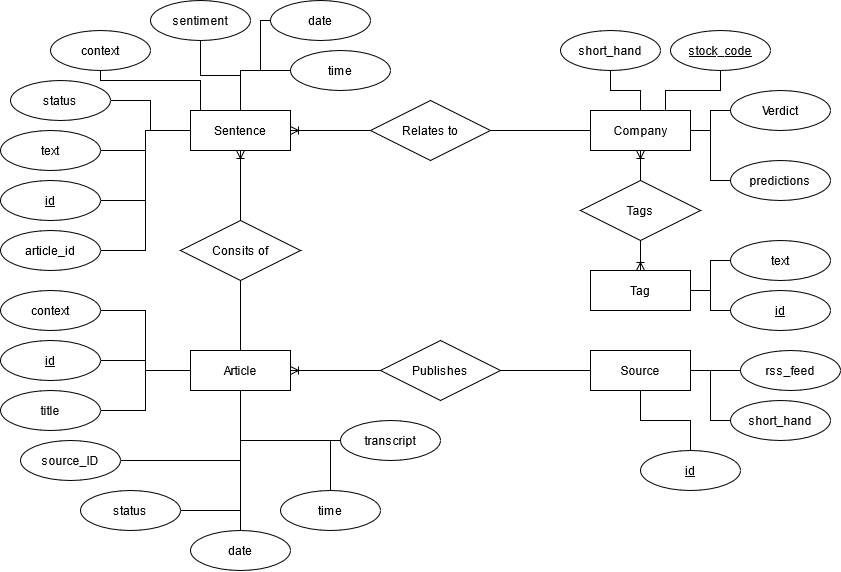
\includegraphics[width=0.7\textwidth]{images/upload/ER full.png}
            \caption{Main Database ER diagram.}
            \label{fig:db_schema_main}
        \end{figure}
        
        Sources are the news sites that articles are gathered from, with every article that is crawled linking to one of these news sources. Each article stores various information such as the time it was crawled, title, article transcript, etc. When sentences are extracted from an article, they are stored in the Sentence table, with each sentence storing its parent article ID, along with its text, sentiment and context. The company table stores the stock code and shorthand of all the companies in the system with various tags and sentences linking to a given company. Additionally, the article and sentence tables were extended to have a 'status' field that links to the current stage of the process of either the article or sentence. The status that an article could take are:
        
        \begin{itemize}
            \item \textbf{Context}, The article is waiting to be processed by the context identification component
            \item \textbf{Sentences}, The article is waiting to have its sentences extracted
            \item \textbf{Done}, The article has been completely analyzed
        \end{itemize}
        
        The various statuses for the sentences are as followed:
        
        \begin{itemize}
            \item \textbf{Context}, The sentence is waiting to be processed by the context identification component
            \item \textbf{Sentiment}, The sentence is waiting to be processed by the sentiment analysis component
            \item \textbf{Pred}, The sentence is waiting to be translated into a data point by the prediction component
            \item \textbf{Done}, the sentence has been completely analyzed
        \end{itemize}
        
        The status field was added for two main reasons. Firstly, it allows for easier lookup of which articles and sentences have been completely analyzed and which have not. Secondly, it supports the control component, \ref{Control Component}, in determining the current of analysis of the given article or sentence. Additionally, both articles and sentences can receive the \textbf{Blocked} status, meaning that during context analysis, no company was registered and as such no more analysis is required. This prevents useless articles and sentences from being processed.  
        
        \subsection{Time-series Database}
        \label{TimeseriesDB}
        % REDONE, sort of
        The prediction component needs to have fast access to the sentiment data for a given company. Although simply querying a sentence's sentiment by a company. and ordering by time would produce the same result, a time-series database would reduce query times significantly. Therefore, it was decided that a separate time-series database containing data points for the perdition component. Data points contain the time the sentence it refers to was crawled, the sentence's ID, sentiment, stock code and company closing price at the time it was crawled. Having a time-series database allows easy lookup and referral to a company's sentiment history with the data already ordered for the components of the prediction.  
       
       
    \section{Frontend}
    The frontend component is the web app that allows the users to view and interact with the data collected on companies. Using inspiration from the competitor sites reviewed in section \ref{Competitors} it was decided that there would be two main pages. A home page, as mentioned in requirement \textbf{\#13}, that presents a shortlist of all the companies on the site along with their \emph{Hot or Not} rating along with a central search bar that allows user to filter and search through the companies. The second page is the company specific that displays relevant information on the company such as stock price, business summary, financial data, etc as well as a graph of previous stock price along with a prediction on the future of the stock price. 
        
        \subsection{Prototypes}
        Before implementation of the frontend, a series of wireframes were developed in an iterative process for the two pages on the webapp. This ensured that all requirements were represented and accounted for in the design of the webpage. 
        
        \subsubsection{Homepage}
        \label{Homepage}
        The Homepage is the first place a user will land when going to the website and therefore required careful planning on the design and layout of the page. Additionally, the page must be able to fulfil requirement \textbf{\#15} by having a search bar to find companies and requirements \textbf{\#19} and \textbf{\#16}, by having tags and filter options for searching.
        
        \begin{figure}[!h]
            \begin{subfigure}[b]{0.4\textwidth}
                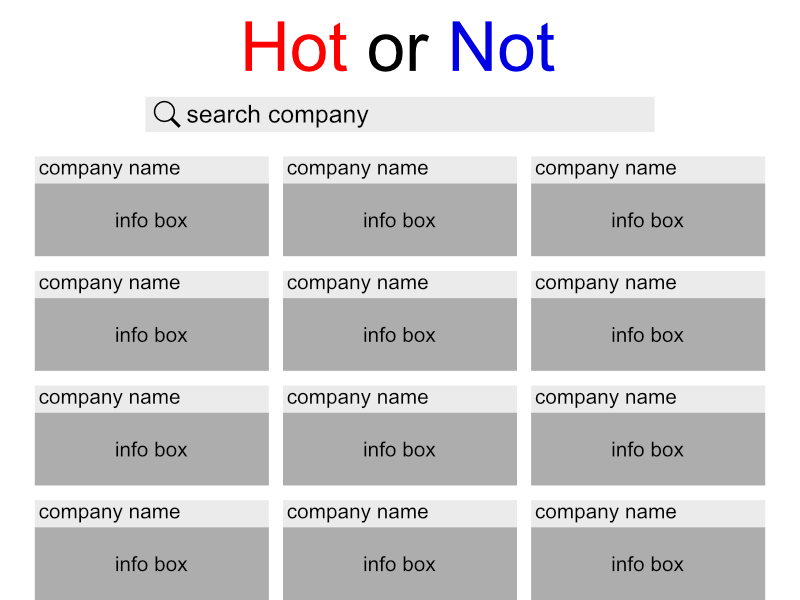
\includegraphics[width=\textwidth]{images/upload/Home Wireframe.png}
                \caption{Initial wireframe.}
                \label{fig:homepage_initial}
            \end{subfigure}
            \hfill
            \begin{subfigure}[b]{0.4\textwidth}
                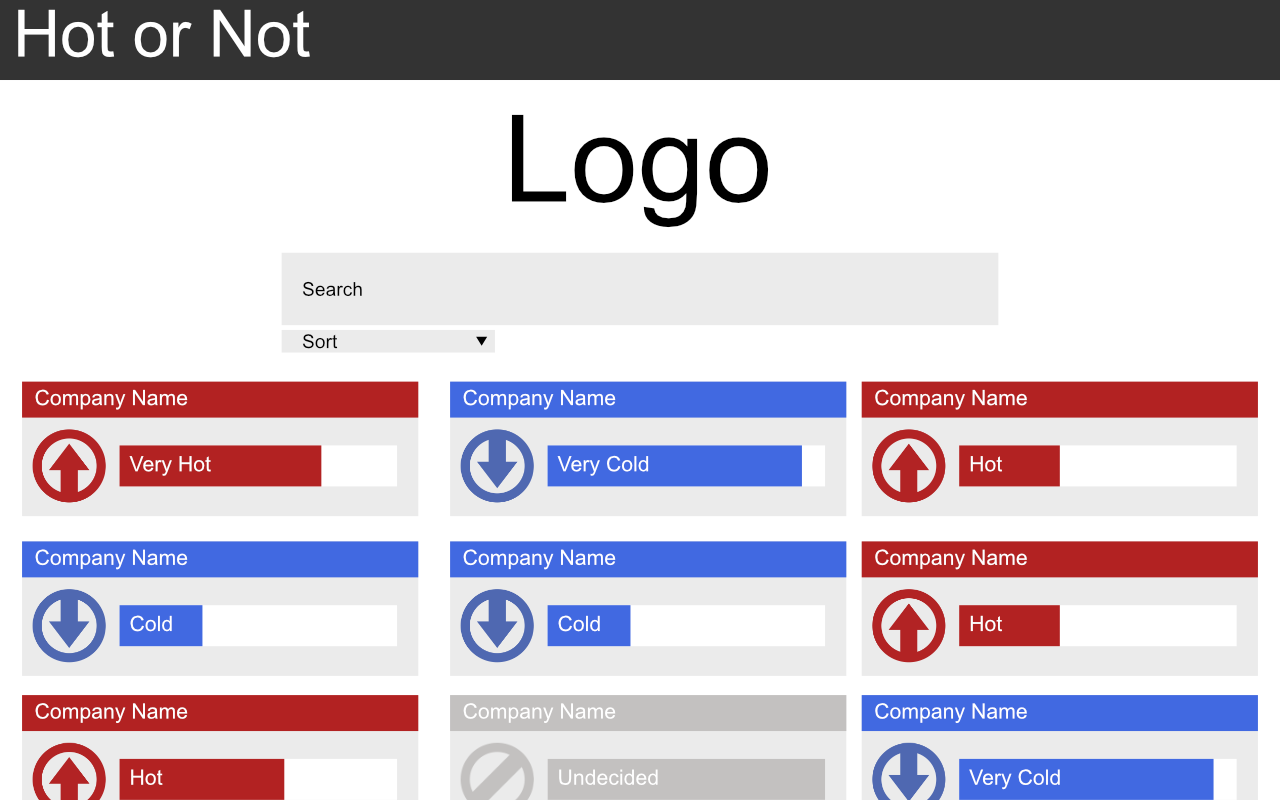
\includegraphics[width=\textwidth]{images/upload/Home-wireframe2.png}
                \caption{Revised wireframe.}
                \label{fig:hompage_revised}
                \end{subfigure}
            \caption{Homepage wireframes}
        \end{figure}
        
        A minimalist design was desired that showed the user enough information to make meaningful assumptions on a company just from a glance at the homepage but wouldn't show too much information and over-complicate or overcrowd the homepage. The initial design of the company page shown in figure \ref{fig:homepage_initial} began the idea of having small information boxes for each company along with the ability to search through these information boxes through a search bar at the top of the screen. This design was then expanded, shown in figure \ref{fig:hompage_revised} by having a Hot to Not meter for each company, giving an indication of how well each company is predicted to perform without complicating the design. Moreover, the search bar was made a larger and more prevalent part of the homepage, along with a colour scheme and icons for each potential verdict a company could receive; Hot, Not or Hold. 
        
        \subsubsection{Company Page}
        The company page allows the user to see information on a given company and contains many critical requirements that must be completed for the system and project to succeed. The wire frames for the company page started with layout, see Figure \ref{fig:Company_itsss} and how the core sections of the company page should fit together. For requirement \textbf{\#22} the company page had to show the different sentences found on the given company and deciding where this should be placed was one of the difficulties when designing the company page. Iteration \ref{fig:company_it3} was finally elected to build upon further as it was felt it provided a simplistic layout and didn't emphasise the article snippets while also giving them the screen space they needed
          
        \begin{figure}[!h]
            \begin{subfigure}[b]{0.3\textwidth}
                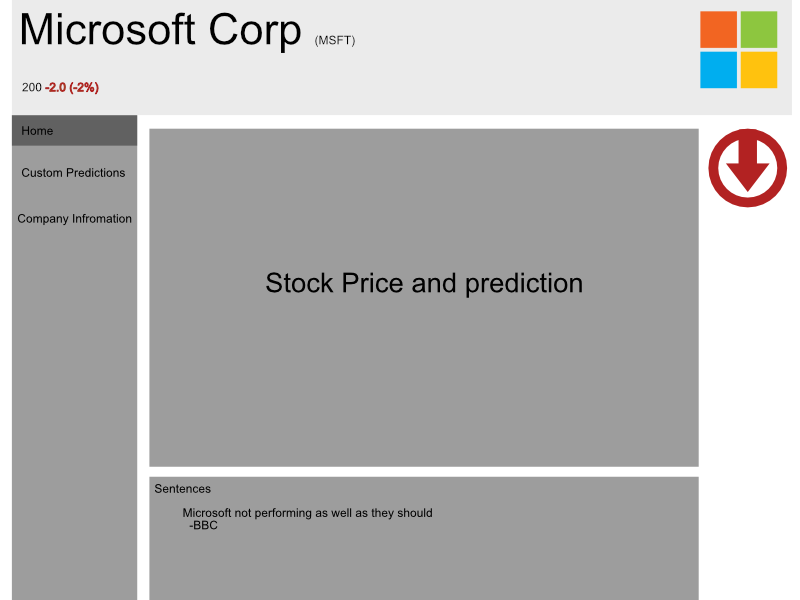
\includegraphics[width=\textwidth]{images/upload/Company-Wireframe1.png}
                \caption{Iteration One.}
                \label{fig:company_it1}
            \end{subfigure}
            \hfill
            \begin{subfigure}[b]{0.3\textwidth}
                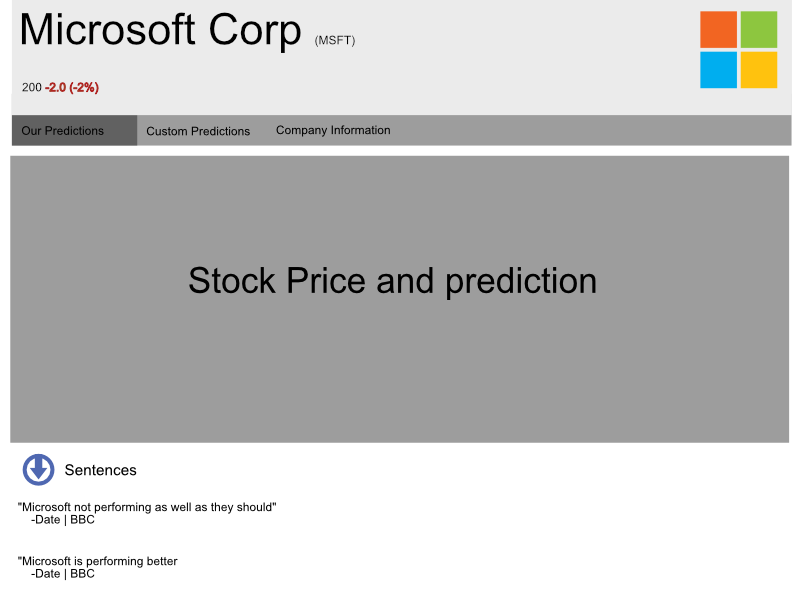
\includegraphics[width=\textwidth]{images/upload/Company Wireframe 3.png}
                \caption{Iteration Two.}
                \label{fig:company_it2}
            \end{subfigure}
            \hfill
            \begin{subfigure}[b]{0.3\textwidth}
                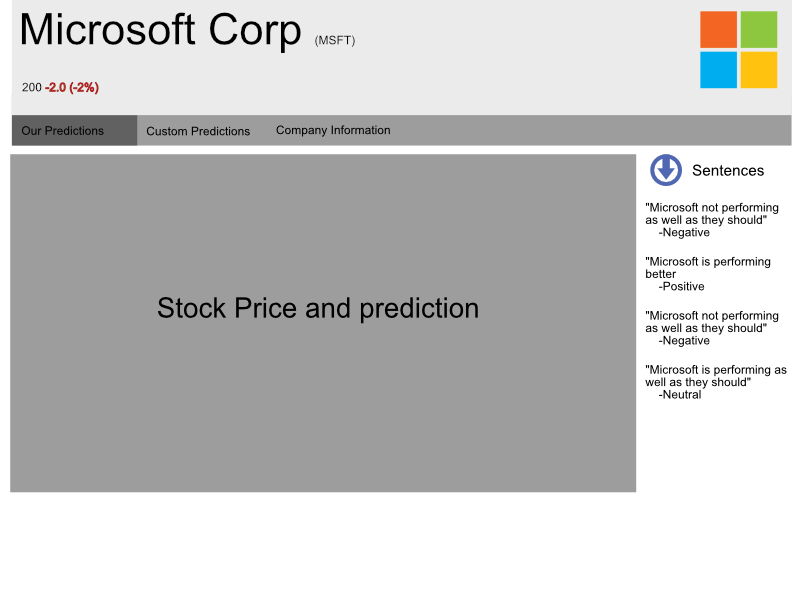
\includegraphics[width=\textwidth]{images/upload/Company Wireframe 2.png}
                \caption{Iteration Three.}
                \label{fig:company_it3}
            \end{subfigure}
            \caption{Company page wireframe iterations}
            \label{fig:Company_itsss}
        \end{figure}
        
        The next task was to design how each tab on the company page should be laid out. The prediction tab shown in Figure \ref{fig:company_tab1} is where systems default prediction for the stock price is shown and gives a graph of the previous prices thus ensuing requirements \textbf{\#18} and \textbf{\#17} are represented. The information tab shown in Figure \ref{fig:company_tab2} was added, in order to fulfil requirement \textbf{\#21} and is home to general information about the company, such as the company's logo, sector and financial information. The final tab shown in Figure \ref{fig:company_tab3} is where users can create custom predictions for the company's stock price by telling the system what start and end date should be used.
        
        \begin{figure}[!h]
            \begin{subfigure}[b]{0.3\textwidth}
                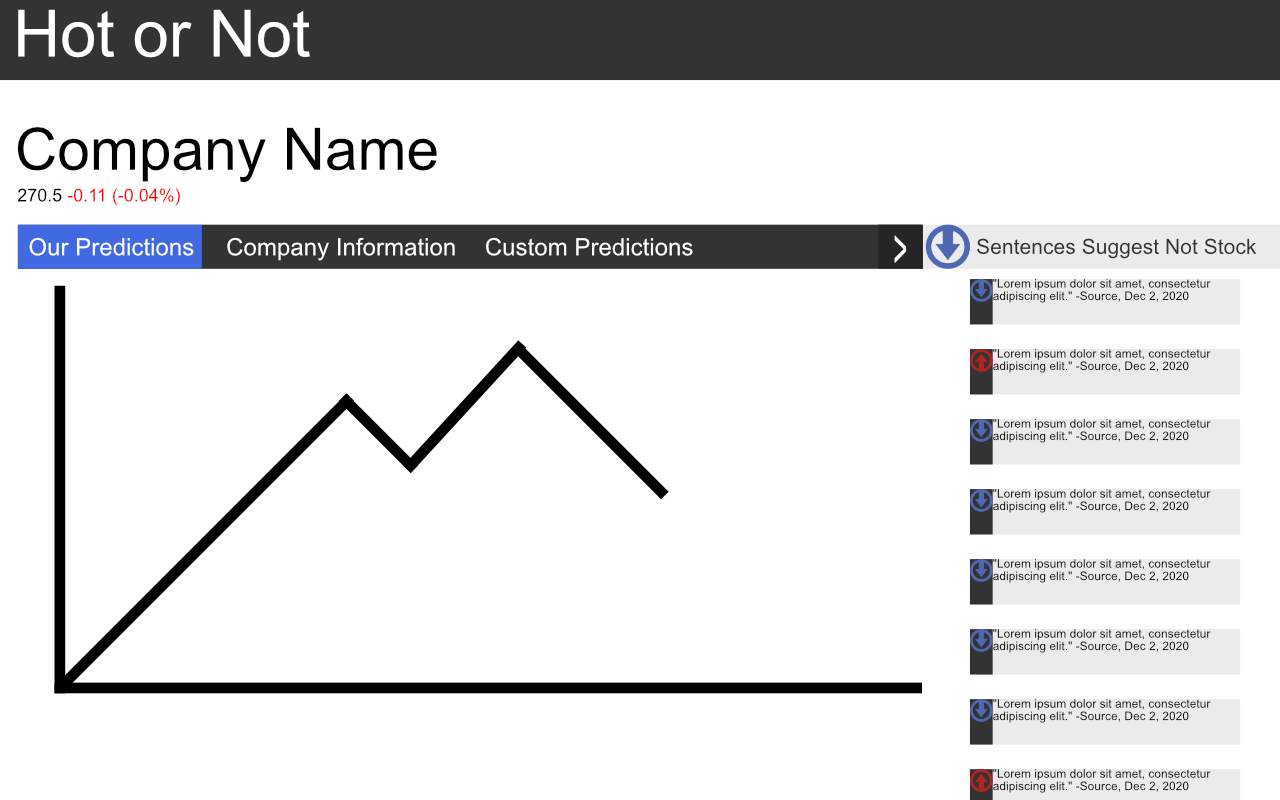
\includegraphics[width=\textwidth]{images/upload/Company-wireframe 4.png}
                \caption{Prediction Tab.}
                \label{fig:company_tab1}
            \end{subfigure}
            \hfill
            \begin{subfigure}[b]{0.3\textwidth}
                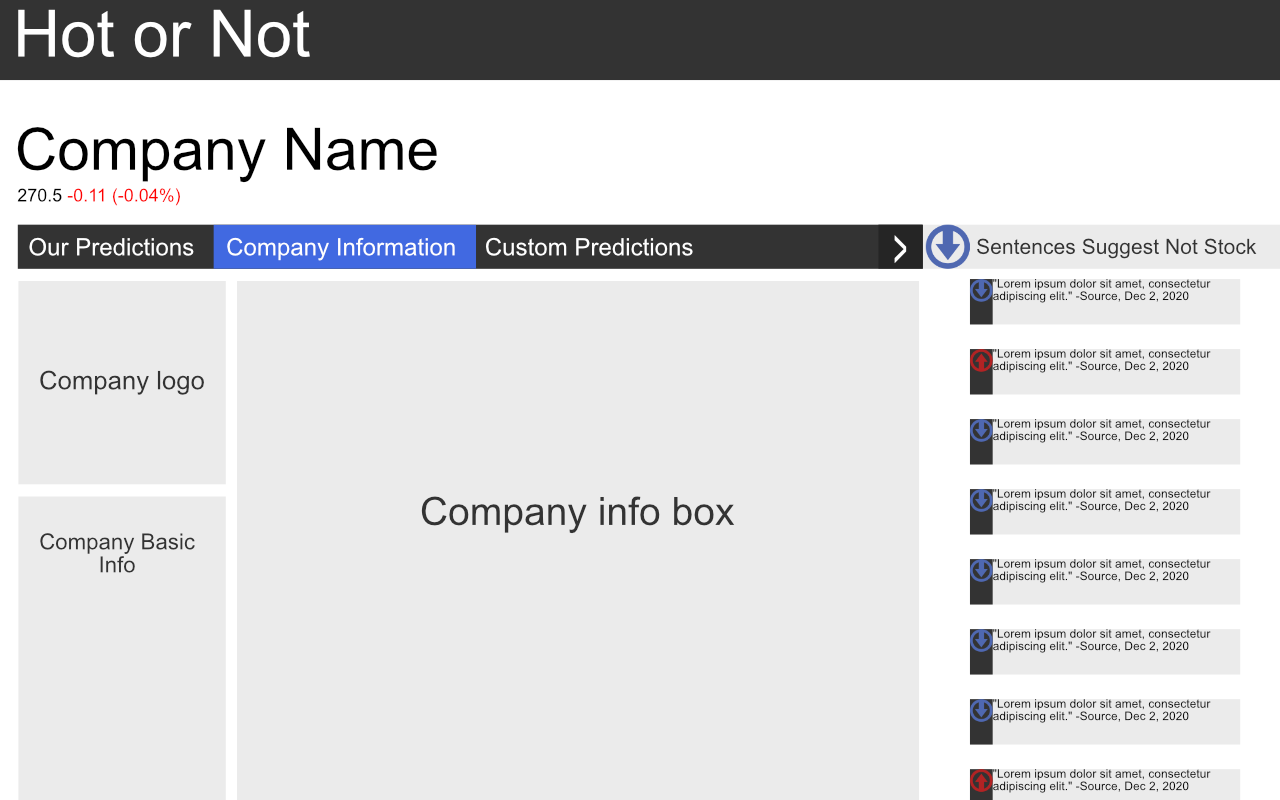
\includegraphics[width=\textwidth]{images/upload/Comapny-wireframe 6.png}
                \caption{Information tab}
                \label{fig:company_tab2}
            \end{subfigure}
            \hfill
            \begin{subfigure}[b]{0.3\textwidth}
                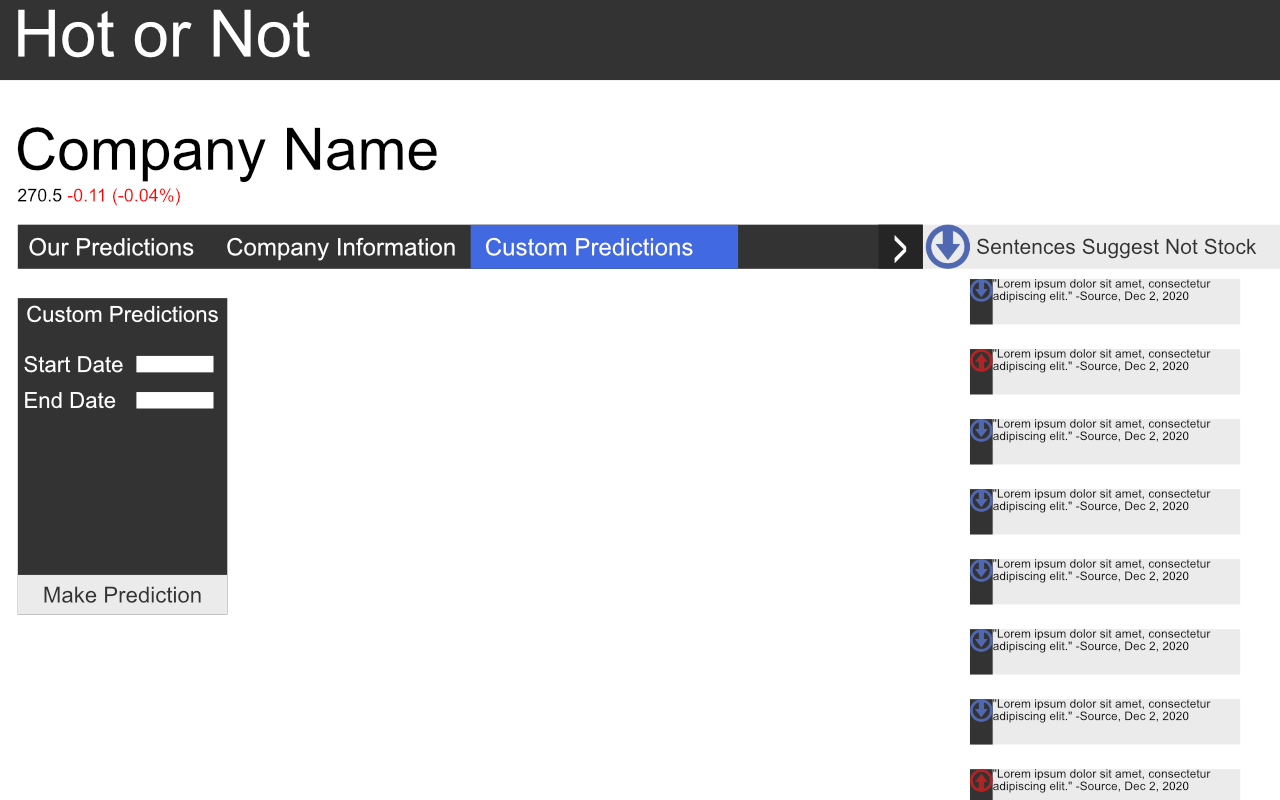
\includegraphics[width=\textwidth]{images/upload/Company-wireframe 5.png}
                \caption{Custom Prediction tab}
                \label{fig:company_tab3}
            \end{subfigure}
            \caption{Company page separate tab wireframes}
        \end{figure}
        
    \section{Summary}
    This chapter highlights and justifies the design decisions made in regards to the project. An overview of the system's architecture along with a description of the operation and purpose of each component is provided. The design choices and overview of the database system along with the process for designing the frontend through an iterative wireframe approach was also detailed. 